\subsection{Definitions and Key Concepts}

\subsection{Architecture and Framework}

In \cite{etsi_ref_003}, the \gls{etsi} defines the framework and architecture for the deployment of \gls{mec}, including its key components, reference points, and interfaces necessary to enable edge computing capabilities at the edge of mobile networks. As illustrated in Figure \ref{fig:mec_etsi_arch}, this MEC system reference architecture consists of several functional entities divided into two levels: the MEC System and MEC Host Levels.

The System Level includes critical components such as the Multi-access Edge Orchestrator (MEO), User Application Lifecycle Management Proxy (UALMP), and Operations Support System (OSS). The MEO serves as the core orchestration entity, maintaining a comprehensive view of the entire MEC system, including the available resources, services, and topology. It coordinates the deployment of applications across multiple MEC hosts based on the requirements, constraints, and available resources. The UALMP acts as an intermediary for user application instantiation requests, whereas the OSS interfaces with the MEC system for operational and business support functions. 

At the Host Level, key components include the MEC Platform Manager (MEPM), MEC Platform (MEP), Virtualization Infrastructure Manager (VIM), and Virtualization Infrastructure itself. The MEPM oversees the management of the MEC platform and applications within a specific MEC host and works in coordination with the MEO at the System Level. The MEP provides an execution environment for MEC applications and offers a set of services and APIs that applications can leverage. The Virtualization Infrastructure, managed by the VIM, provides the computing, storage, and network resources required for hosting MEC applications and platform components.

\begin{figure}[h]
    \centering
    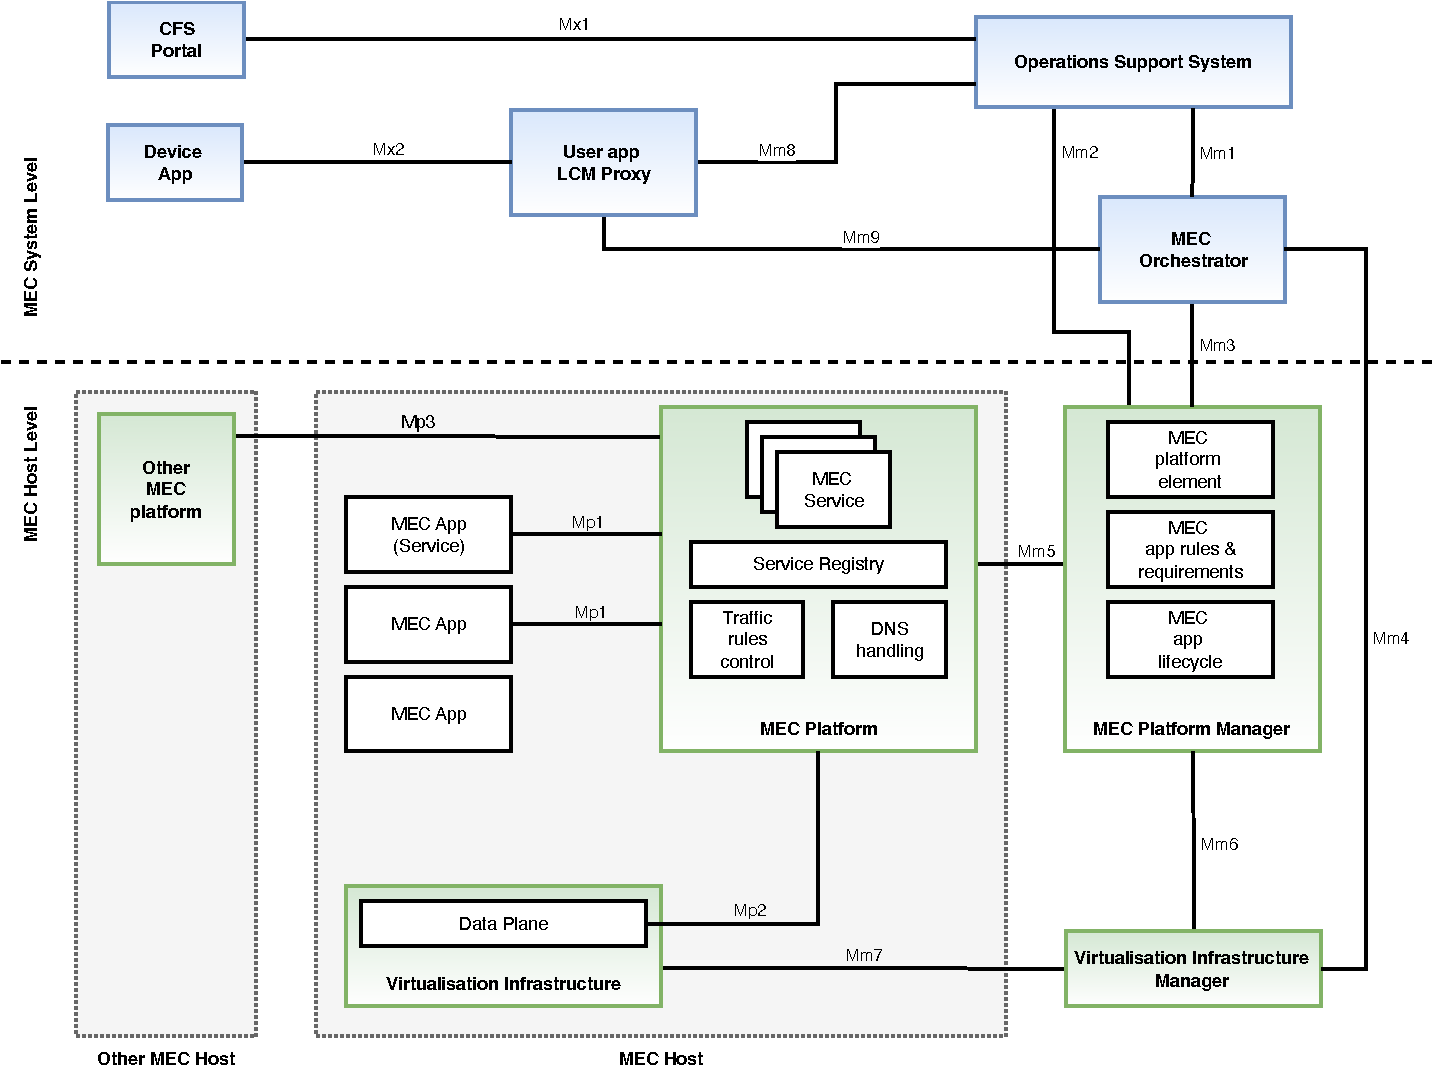
\includegraphics[width=1\linewidth]{Chapters/Figures/Diagrams/etsi_ref_003.pdf}
    \caption{MEC ETSI system reference architecture.}
    \label{fig:mec_etsi_arch}
\end{figure}

\subsection{Use Cases}
% passar para secção

